\documentclass[11pt]{article}

\usepackage[margin=1in]{geometry}
\usepackage{setspace}
\usepackage{amsmath,amssymb}
\usepackage{graphicx}
\usepackage{booktabs}
\usepackage{hyperref}
\usepackage{enumitem}

\setstretch{1.15}
\setlength{\parskip}{0.5em}
\setlength{\parindent}{0pt}

\title{\textbf{False-positive-resistant nonlocal diagnosis of field-free topological superconductivity in compensated-magnetic Josephson junctions}}
\author{Author A, Author B, Author C\\
\small [Affiliations to be inserted]}
\date{}

\begin{document}
\maketitle

\begin{abstract}
Field-free routes to topological superconductivity are attractive because strong magnetic fields and ferromagnetic stray fields can compromise proximity-induced pairing and complicate spectroscopic interpretation. Yet local near-zero-energy features alone do not distinguish Majorana end modes from trivial Andreev or impurity-induced states. Here we study a phase-biased Josephson junction with a compensated magnetic weak link, in which momentum-dependent spin splitting drives a bulk gap closing and a $Z_2$ topological transition without net magnetization. We show that trivial near-zero states can be generated by local impurities and weak disorder, but they fail a combined diagnostic based on bulk topology, boundary-state isolation and phase-resolved nonlocal transport. The resulting criterion provides a false-positive-resistant route for identifying field-free topological superconductivity in compensated-magnetic superconducting devices.
\end{abstract}

% Submission draft note:
% 1. Before submission, verify that the title, abstract, Fig. 5 caption, and Discussion
%    all use the same contribution line: false-positive-resistant nonlocal diagnostic.
% 2. Keep claims such as "universal", "model-agnostic", or "optimal" out of the main text
%    unless new evidence is added and mirrored in the Supplement.

\section{Introduction}

Field-free routes to topological superconductivity are becoming increasingly important because the magnetic fields commonly used to drive Majorana platforms can also suppress proximity-induced pairing, introduce orbital complications and blur spectroscopic interpretation. This tension is especially acute in Josephson-based architectures, where phase control offers an attractive tuning knob but where the absence of a clean magnetic-field-free diagnostic has limited how convincingly low-energy boundary features can be interpreted. The field therefore needs not only additional candidate platforms, but also stricter ways to determine when a field-free low-energy state is genuinely topological.

That need remains unmet. Local zero-bias or near-zero-energy signatures are now understood to be intrinsically ambiguous because trivial Andreev bound states, impurity-induced in-gap states and weak-disorder resonances can all generate similar low-energy features. At the same time, recent planar and compensated-magnetic Josephson-junction proposals have sharpened the platform landscape without resolving the central exclusion problem: how to identify topology without relying on a local near-zero mode alone. As a result, the limiting issue is no longer whether one can engineer another putative field-free junction, but whether one can impose an experimentally relevant false-positive filter on the resulting low-energy states.

Here we study a phase-biased Josephson junction with a compensated magnetic weak link that produces momentum-dependent spin splitting without net magnetization. In this setting, superconducting phase bias acts as the control parameter that drives a bulk gap closing and reopening together with a $Z_2$ topological transition. This makes the junction a useful arena for separating platform novelty from diagnostic rigor: the compensated magnetic texture supplies a field-free route to the transition, while the phase dependence allows the bulk, boundary and transport responses to be compared on the same footing. The key question is therefore not whether a near-zero mode can appear, but whether all physically relevant observables point to the same topological window.

We answer that question by constructing a closed evidence chain. We first identify the bulk topological transition from the gap closing and $Z_2$ invariant. We then show that open-boundary near-zero modes become meaningful only when they are spectrally isolated and end-localized in the same phase window. Next, we introduce explicit impurity and disorder controls to test whether trivial low-energy states can mimic the boundary signal. Finally, we show that a phase-resolved nonlocal transport response survives these false-positive tests and provides the operational discriminator missing from local spectroscopy alone. We therefore identify topology not from the appearance of a near-zero mode, but from the consistency of bulk topology, boundary spectra and phase-resolved nonlocal response under controlled false-positive tests.

% Reference placeholders for Introduction:
% [Ref-I1] field-free / low-stray-field motivation
% [Ref-I2] ambiguity of local zero-bias or near-zero features
% [Ref-I3] recent planar Josephson-junction proposal
% [Ref-I4] recent compensated-magnetic / TAJJ proposal
% [Ref-I5] diagnostic ambiguity / false-positive literature

\section{Results}

\subsection{Bulk topology is driven by phase bias in the absence of net magnetization}

We begin by establishing the bulk transition that underlies the rest of the manuscript. In the compensated-magnetic junction, the magnetic texture generates momentum-dependent spin splitting while preserving zero net magnetization, so the relevant control parameter is not a conventional Zeeman field but the superconducting phase bias. Figure~2 shows that varying $\phi$ drives a bulk gap closing and reopening over a finite parameter window, and that this spectral transition is accompanied by a simultaneous change in the $Z_2$ invariant. This alignment is essential: the reopening is not treated as a generic low-energy rearrangement, but as the point at which the bulk diagnosis changes from trivial to topological. The phase-biased compensated-magnetic junction therefore provides a field-free route to a topological transition whose location can be identified directly from bulk quantities before any appeal is made to boundary spectroscopy.

\begin{figure}[t]
\centering
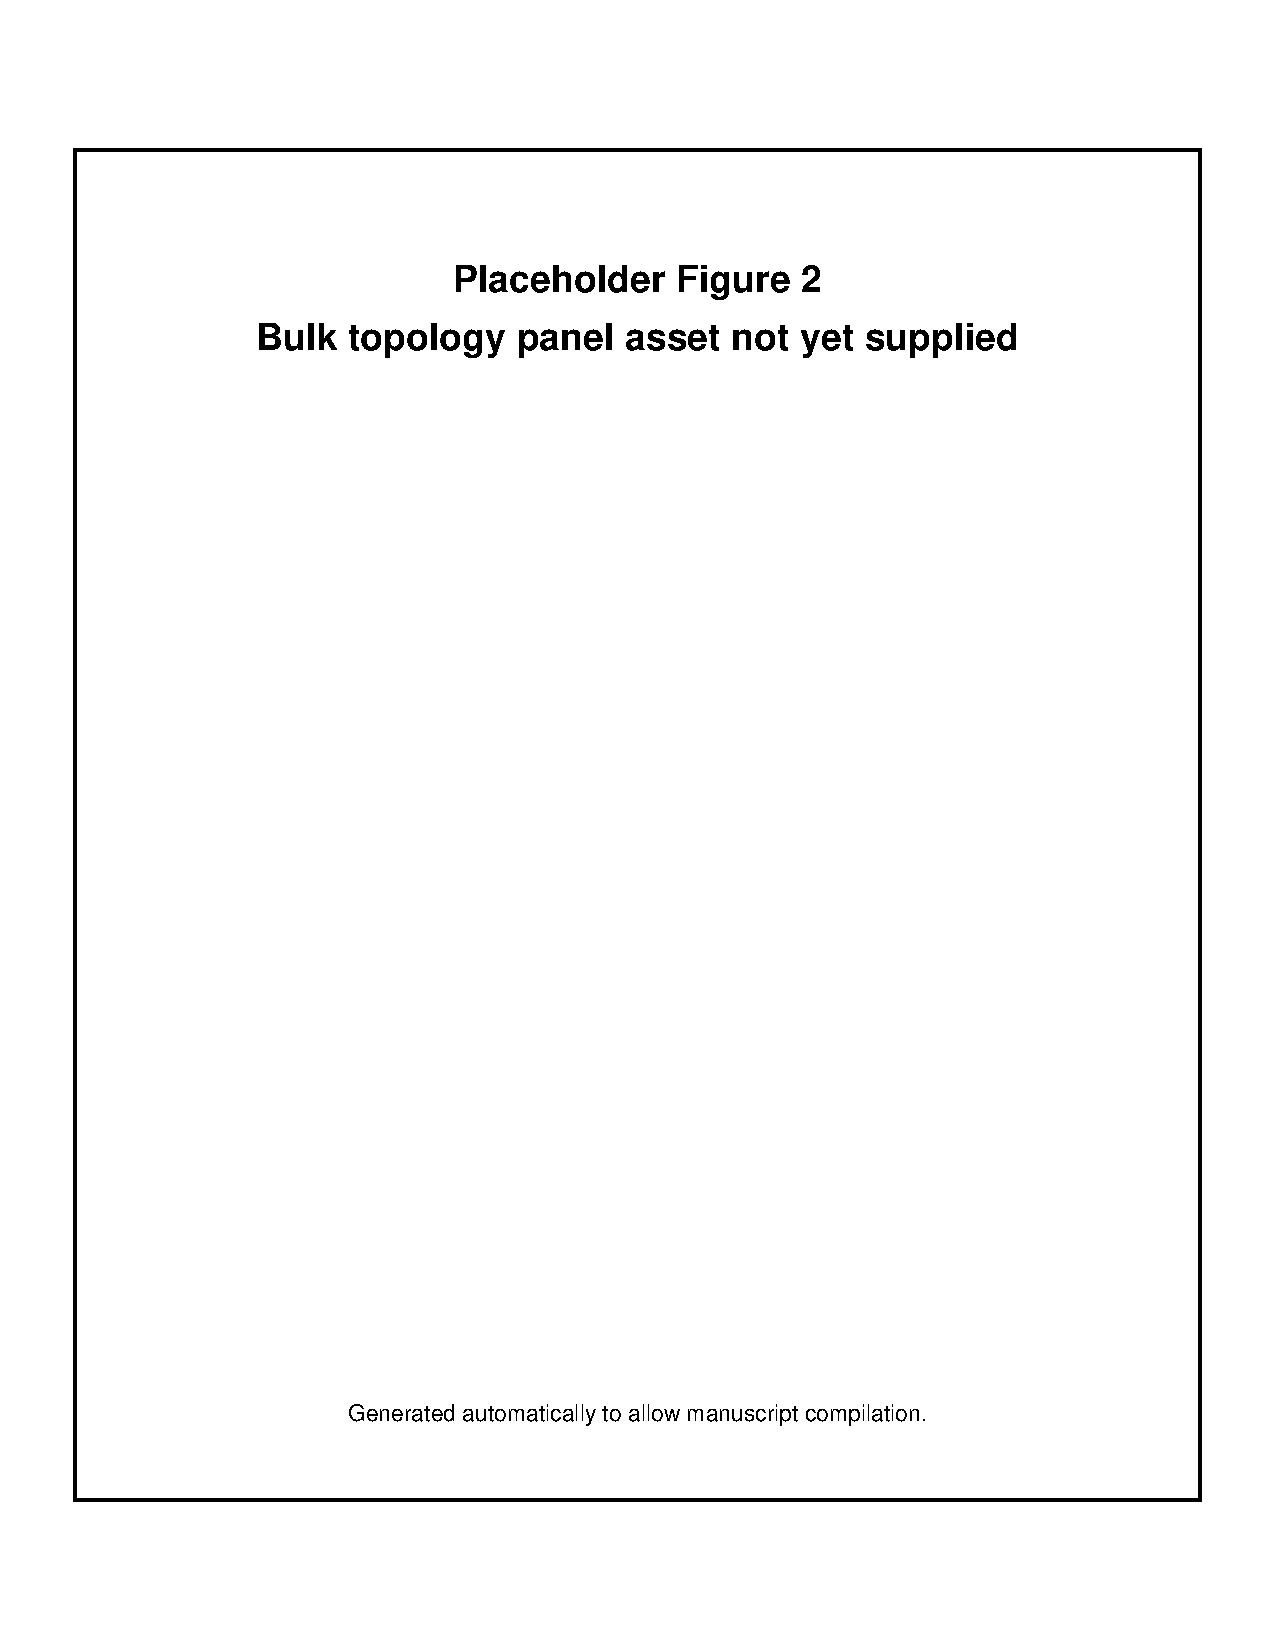
\includegraphics[width=\textwidth]{figures/Fig2_bulk_topology.pdf}
\caption{\textbf{Phase-driven bulk topological transition without net magnetization.} This figure shows that superconducting phase bias drives a bulk topological transition in the absence of a conventional Zeeman field. \textbf{a,} Normal-state band splitting generated by the compensated magnetic texture, highlighting finite momentum-dependent spin splitting at zero net magnetization. \textbf{b,} Bulk excitation gap as a function of phase bias and chemical potential, revealing a gap closing and reopening that marks the transition between trivial and topological regimes. \textbf{c,} Corresponding $Z_2$ topological invariant over the same parameter space, showing that the gap reopening coincides with a change in bulk topology rather than a crossover between spectrally similar trivial states. \textbf{d,} Representative cut at fixed magnetic texture strength, resolving the gap minimum and reopening across the transition. Together, these panels establish that field-free topology in this junction is controlled by the interplay of compensated magnetic splitting, induced pairing and phase bias, and that the bulk transition can be identified independently of boundary spectroscopy.}
\label{fig:bulk-topology}
\end{figure}
% Source-data placeholder: source_data/Fig2/

\subsection{Boundary near-zero modes emerge in the topological window, but zero energy alone remains ambiguous}

We next turn to the open-boundary spectrum to determine what the bulk transition implies for low-energy boundary structure. As shown in Fig.~3, a near-zero branch appears only after entering the topological phase window identified from the bulk calculation, and representative wavefunction profiles on that side of the transition show weight concentrated at opposite ends of the junction. Taken alone, however, this observation is still insufficient. Trivial parameter choices or local perturbations can also generate low-energy boundary features that approach zero energy without carrying the same topological meaning. For this reason, we do not identify the topological branch by zero energy alone. Instead, the relevant boundary signature is the coexistence of near-zero energy, end localization and spectral isolation within the same phase window selected independently by the bulk transition. Figure~3 therefore plays a narrowing role rather than a concluding one: it shows what a candidate topological boundary mode should look like, while making explicit why local low-energy structure cannot serve as a sufficient criterion.

\begin{figure}[t]
\centering
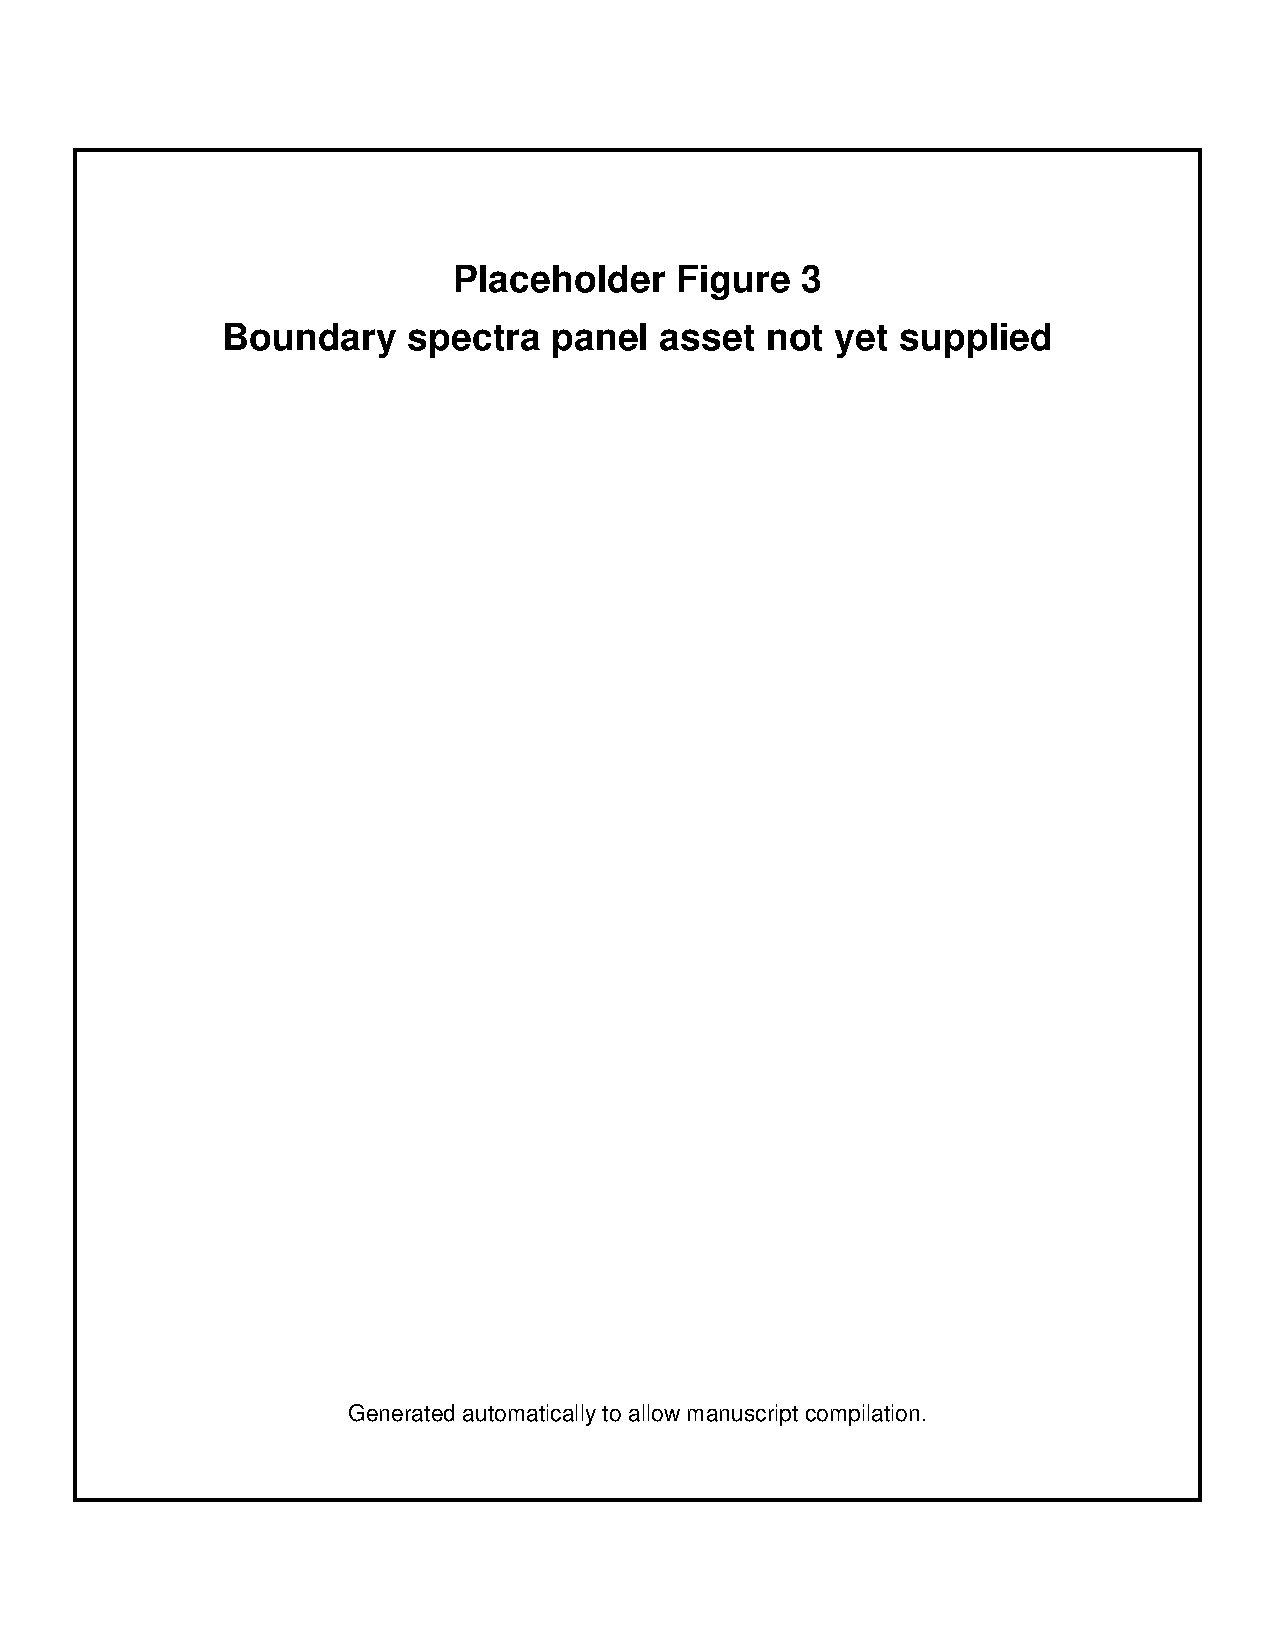
\includegraphics[width=\textwidth]{figures/Fig3_boundary_spectra.pdf}
\caption{\textbf{Boundary spectra reveal near-zero modes, but zero energy alone does not identify topology.} This figure separates genuine topological boundary modes from trivial near-zero mimics. \textbf{a,} Open-boundary spectrum versus phase bias, showing the emergence of a near-zero branch only after the bulk transition identified in Fig.~2. \textbf{b,} Spatial profile of the low-energy state in the topological regime, with weight localized at opposite ends of the junction, consistent with a nonlocal boundary mode. \textbf{c,} Counterexample from a trivial parameter regime or local perturbation, where a near-zero state appears but remains spatially asymmetric or insufficiently isolated from the low-energy background. \textbf{d,} Spectral-isolation metric for the lowest mode, demonstrating that the topological branch is distinguished not by zero energy alone, but by simultaneous end localization and clean separation from nearby trivial states. These results motivate the stricter claim used in the main text: local near-zero structure is necessary but not sufficient, and boundary spectroscopy must be interpreted together with bulk topology and nonlocal transport.}
\label{fig:boundary-spectra}
\end{figure}
% Source-data placeholder: source_data/Fig3/

\subsection{Negative controls show that trivial low-energy mimics survive local tests but fail the full evidence chain}

The ambiguity of local spectroscopy becomes most useful when it is converted into a null test rather than a qualitative caution. We therefore evaluate explicit trivial null ensembles, generated in bulk-trivial regimes with either local impurity perturbations or weak disorder, under the same prespecified diagnostic rule used for the topological ensemble. Figure~4 is organized around this comparison. The first point is that the null can indeed generate local near-zero mimics: trivial samples can acquire low-energy structure that would be misleading if judged only by local spectra or selected wavefunction profiles. The second, and more important, point is that these null realizations remain quantitatively separated from the topological ensemble once the full diagnostic score is evaluated at the distribution level.

This separation is not presented as a visual impression alone. Instead, we compare the topological and null ensembles through a fixed scalar diagnostic outcome and report both the associated effect size and the null-calibrated false-positive rate. The relevant question is therefore not whether some trivial samples can look superficially similar, but whether the topological ensemble remains distinguishable from impurity-driven and disorder-driven trivial ensembles after uncertainty is taken into account. Figure~4 shows that it does: the topological ensemble occupies a distinct score distribution, while the null ensembles remain confined to the expected false-positive background band. In this form, the control analysis becomes a quantitative falsification step rather than a gallery of counterexamples.

\begin{figure}[t]
\centering
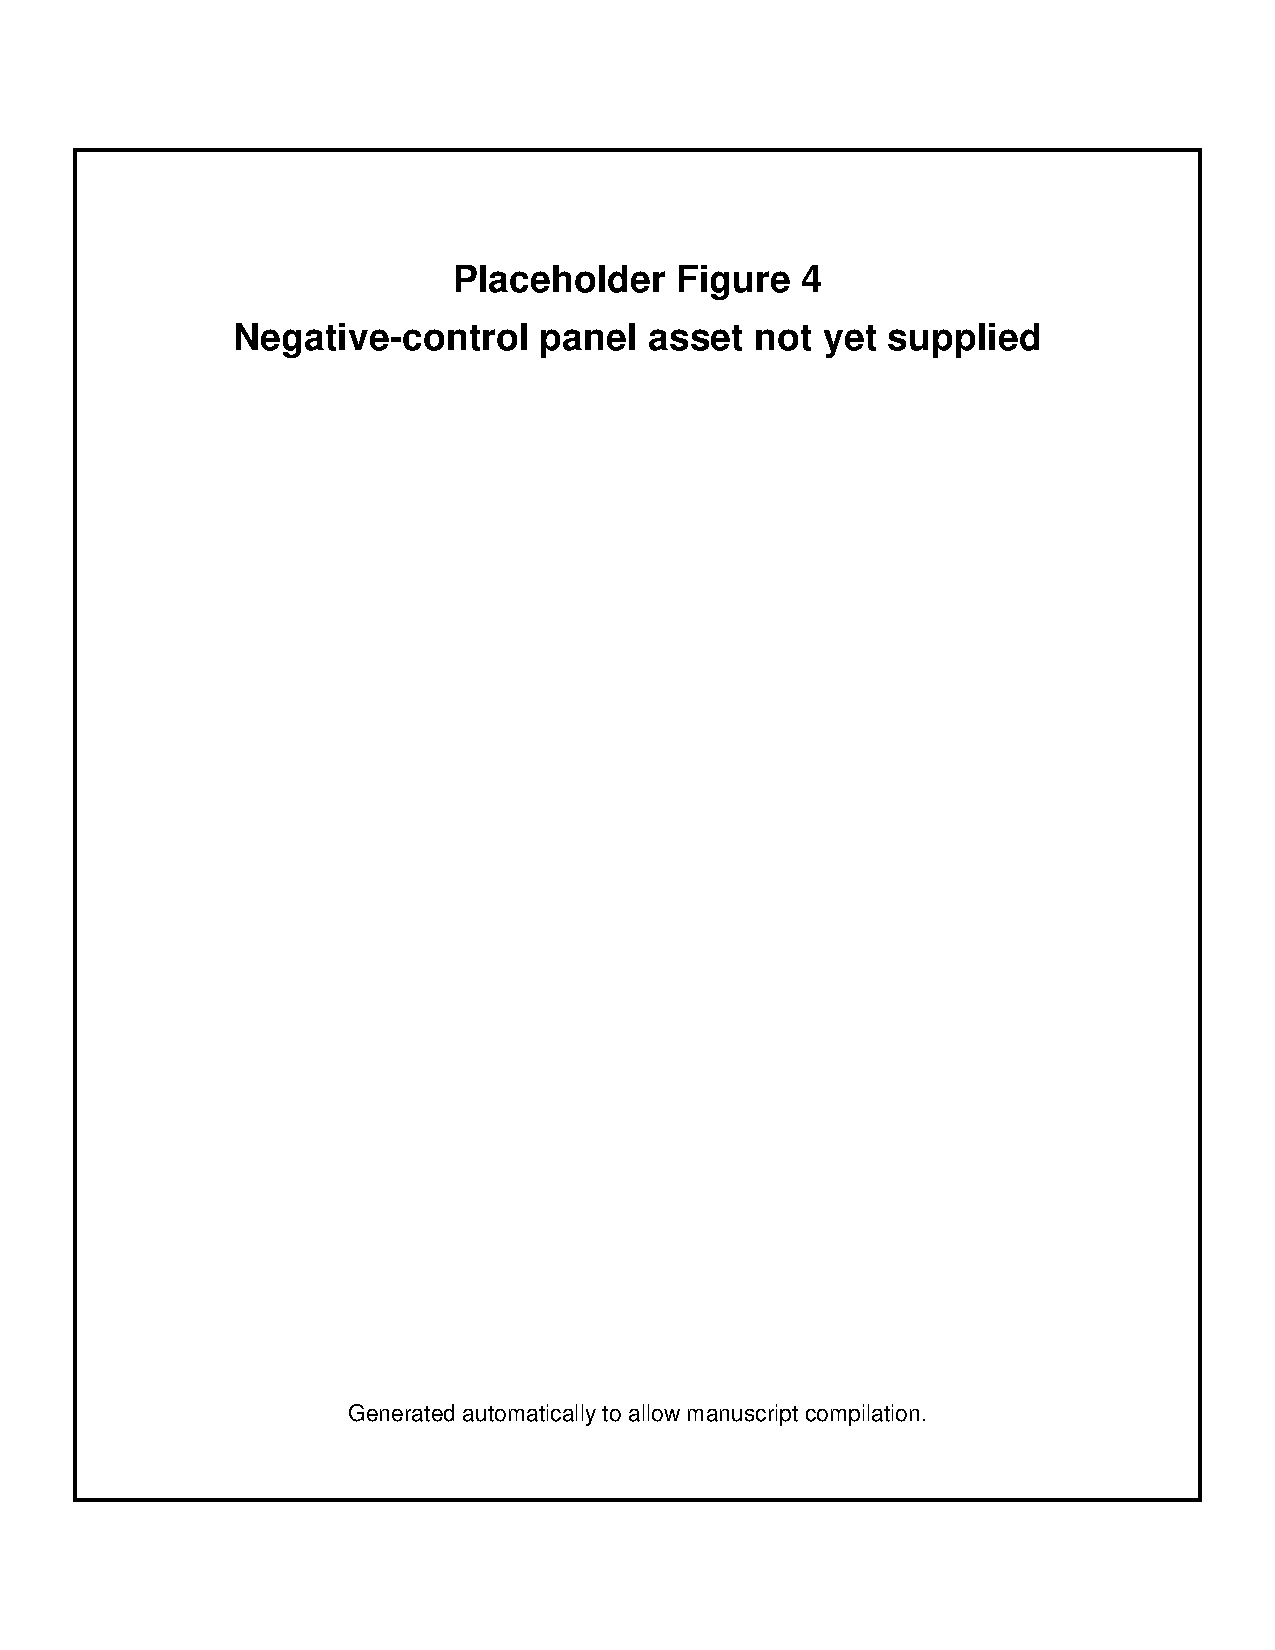
\includegraphics[width=\textwidth]{figures/Fig4_negative_controls.pdf}
\caption{\textbf{Null-calibrated controls show that trivial near-zero mimics fail the diagnostic at the distribution level.} This figure tests the diagnostic against prespecified trivial null ensembles rather than selected counterexamples. \textbf{a,} Local impurity and weak-disorder perturbations applied in a bulk-trivial regime generate near-zero spectral mimics despite the absence of a topological transition. \textbf{b,} Distribution of the final diagnostic score across topological, impurity-generated trivial and disorder-generated trivial ensembles, showing that local mimics do not reproduce the same ensemble-level behavior as the topological branch. \textbf{c,} Effect-size summary, with bootstrap confidence intervals, quantifying the separation between the topological ensemble and the two null ensembles. \textbf{d,} Empirical true-positive and false-positive rates for the prespecified pass criterion, demonstrating that the trivial null ensembles remain confined to the expected background failure band. \textbf{e,} Stability of the null separation under variation of nuisance parameters such as impurity strength, disorder amplitude or thermal broadening. The figure therefore shows not only that trivial perturbations can mimic local low-energy features, but that they fail the final diagnostic in a statistically calibrated sense.}
\label{fig:negative-controls}
\end{figure}
% Source-data placeholder: source_data/Fig4/
% Statistical lock for Fig. 4:
% - Define explicit trivial null ensembles before plotting.
% - Report one effect size (preferably Cliff's delta or AUROC) with bootstrap CI.
% - Report empirical TPR / FPR under the fixed diagnostic rule.
% - Do not rely on selected examples once ensemble statistics are available.
% Pre-submission check: replace any single-case control with ensemble statistics if not already done.

\subsection{Phase-resolved nonlocal transport provides the operational discriminator}

Having established both the bulk transition and the limitations of local boundary spectroscopy, we finally ask which observable can be promoted to a genuine decision rule. Figure~5 is designed to answer that question with a single prespecified nonlocal criterion rather than with a family of related transport indicators. We define the criterion from the antisymmetrized lead-resolved conductance and require that it exceed a fixed threshold over a connected phase interval that overlaps the independently computed bulk-topological window. Under this rule, the role of the transport analysis is no longer to display several suggestive structures, but to decide whether the same nonlocal window appears in the clean topological regime and whether it fails under the same evaluation rule in trivial controls.

This locking step is essential. Without it, the transport section would remain vulnerable to the objection that different observables or thresholds might be chosen retrospectively for different cases. Instead, Fig.~5 applies one criterion to all comparisons. The clean junction produces a reproducible nonlocal decision window that coincides with the bulk and boundary window, whereas impurity-driven and disorder-driven trivial cases retain local low-energy structure but fail the same nonlocal rule. Extended Data Fig.~1 then tests whether this decision window survives finite temperature, finite bias broadening and representative geometry variation without redefining the criterion. The contribution of Fig.~5 is therefore not that many transport quantities change near the transition, but that one locked nonlocal rule yields a topological pass/fail decision that is consistent with the rest of the evidence chain and does not reproduce under trivial near-zero mimics.

\begin{figure}[t]
\centering

\includegraphics[width=\textwidth]{figures/Fig5_nonlocal_transport.pdf}
\caption{\textbf{A single phase-resolved nonlocal criterion identifies the topological window and fails under the same rule in trivial controls.} This figure converts the transport response into a single prespecified decision system. \textbf{a,} Definition of the raw lead-resolved nonlocal conductance, the antisymmetrized signal $G^{-}(\phi)$, and the fixed threshold-and-window rule used throughout the figure. \textbf{b,} Raw nonlocal response in the clean junction. \textbf{c,} Extraction of the connected phase window selected by the single nonlocal criterion. \textbf{d,} Comparison between that extracted window and the independently determined bulk-topological window. \textbf{e,} Application of the same locked criterion to impurity-driven and disorder-driven trivial controls, which retain local low-energy structure but fail the nonlocal decision rule. \textbf{f,} Final pass-fail summary, including finite-temperature, finite-bias and geometry perturbations under the same criterion. The figure therefore establishes one operational statement only: the topological regime is identified by a reproducible nonlocal decision window that is fixed before control comparisons and is not reproduced by trivial near-zero mimics.}
\label{fig:nonlocal-transport}
\end{figure}
% Source-data placeholder: source_data/Fig5/
% Method lock for Fig. 5:
% - Define one nonlocal decision criterion only.
% - Apply the same threshold and overlap rule to clean and trivial controls.
% - Move all alternative indicators or threshold sweeps to the Supplement.
% Pre-submission check: Fig. 5 must end on one operational criterion, not multiple competing indicators.
% Pre-submission check: finite-T / finite-bias / geometry robustness must support the exact wording used here and in the cover letter.

\section{Discussion}

The main implication of these results is not simply that a compensated-magnetic Josephson junction can host field-free topological superconductivity, but that such a platform can be interrogated by a sharper diagnostic standard than local spectroscopy alone. This distinction matters because the bottleneck in the present field is no longer the absence of candidate low-energy platforms. Rather, it is the difficulty of excluding trivial low-energy mimics once local near-zero structure appears. By aligning bulk topology, open-boundary spectra, explicit negative controls and phase-resolved nonlocal transport on the same phase window, the present analysis shifts the focus from platform plausibility to diagnostic closure.

This is also the sense in which the nonlocal transport result should be interpreted. We do not claim that nonlocal response by itself constitutes a universal proof of topology across arbitrary device classes. Instead, within the compensated-magnetic phase-biased junction studied here, the nonlocal signal functions as the operational observable that remains consistent with the independently determined bulk and boundary windows while trivial controls fail the same test. The value of the criterion is therefore comparative and exclusionary: it is stronger than a local near-zero feature because it survives precisely the false-positive scenarios that make local spectroscopy ambiguous.

The results further suggest that field-free Josephson architectures may be especially useful when phase bias can be used as a common axis along which bulk, boundary and transport observables are compared. In that setting, the question is not whether a given low-energy state looks Majorana-like at a single point in parameter space, but whether multiple observables become mutually consistent over a reproducible phase interval. That framing is likely to be more useful for realistic device assessment than a strategy centered on isolated zero-bias features. In this sense, the present work is best viewed as a diagnostic framework for a timely class of junctions, rather than as a claim that the false-positive problem has been solved in full generality.

Several limitations should be stated explicitly. First, the present study is theoretical and numerical, so experimental visibility is inferred through finite-temperature, finite-bias and geometry tests rather than demonstrated in a specific device. Second, the transport criterion is developed for the compensated-magnetic junction class considered here and should not be advertised as model-agnostic without additional cross-platform analysis. Third, the strength of the manuscript depends on the statistical quality of the impurity and disorder controls and on the reproducibility of the source-data and code package. These are not peripheral implementation details; they are part of the evidentiary standard required for the central claim. For that reason, the contribution should be framed as a false-positive-resistant protocol for this junction class, with clearly stated scope and boundary conditions.

Within those limits, the study advances the field in a concrete way. It identifies a field-free route to a bulk topological transition in a compensated-magnetic Josephson junction, shows why local near-zero modes do not close the case, and supplies a lead-resolved nonlocal observable that tracks the same topological window selected independently by bulk and boundary analysis. That combination is the manuscript's real contribution, and it is the level at which the work should be compared with recent Josephson-junction proposals.

% Discussion check:
% Ensure prior-art comparison is handled with citations or a Supplementary comparison table,
% not with unreferenced general claims.

\section{Conclusion}

We have studied a compensated-magnetic Josephson junction in which superconducting phase bias drives a bulk gap closing, reopening and $Z_2$ topological transition without net magnetization. Open-boundary calculations show that near-zero boundary modes emerge in the topological regime, but explicit impurity and disorder controls demonstrate that local low-energy features alone remain insufficient for identification. The key result is that a phase-resolved nonlocal transport response selects the same window identified independently by the bulk transition and isolated boundary spectrum, while trivial near-zero mimics fail the same consistency test. We therefore conclude that, for this class of field-free junctions, topology is most credibly identified not by a local near-zero signature in isolation, but by a false-positive-resistant evidence chain built from bulk topology, boundary-state structure and nonlocal transport.

\section{Methods}

The system is modeled as a phase-biased compensated-magnetic Josephson junction within a Bogoliubov-de Gennes framework, from which we compute the bulk gap and $Z_2$ invariant, the open-boundary spectra with end-localization metrics, and the lead-resolved nonlocal conductance used in the final diagnostic criterion. The main text reports only the definitions and numerical settings required to interpret Figs.~2--5. Full model specification, invariant implementation, open-boundary diagnostics, disorder and impurity statistics, transport details, effective-model analysis, and reproducibility information are provided in the Supplementary Information.

% Methods check:
% Keep the main-text Methods to one compact page if possible.
% Move failed indicators, alternative classifiers, and large parameter archives to the Supplement.

\subsection{Main-text Methods boundary}

The main-text Methods should remain compact because the manuscript's claim is not methodological novelty in every numerical ingredient. The novelty lies in how these ingredients are combined into a false-positive-resistant evidence chain. The main text should therefore retain only the model definition, the bulk and boundary observables, the transport observable, and the minimal numerical settings needed for interpretation. Full derivations of the topological invariant, detailed convergence tables, alternative transport indicators, complete ensemble bookkeeping and reproducibility manifests belong in the Supplement.

\section*{Figure captions}

\paragraph{Figure 1 \textbar{} Diagnostic logic for field-free topology in a compensated-magnetic Josephson junction.}
This figure defines the physical setting and the diagnostic standard used throughout the manuscript. \textbf{a,} Schematic of a phase-biased Josephson junction formed by two s-wave superconducting leads coupled through a compensated-magnetic weak link, with left and right transport probes used to resolve local and nonlocal response. \textbf{b,} Illustration of momentum-dependent spin splitting in the compensated magnetic region: the spin texture changes sign in momentum space while the net magnetization remains zero, distinguishing this mechanism from a conventional Zeeman field. \textbf{c,} Local near-zero-energy features can arise from both topological and trivial states, so a zero-bias or near-zero spectral feature alone is not a sufficient diagnostic. \textbf{d,} Workflow of the combined criterion used here: bulk topological transition, open-boundary spectra, negative-control tests and phase-resolved nonlocal response must be mutually consistent before a near-zero state is identified as topological. The central claim of the study is therefore not the appearance of a near-zero mode by itself, but the closure of this full evidence chain under controlled false-positive tests.

\paragraph{Figure 2 \textbar{} Phase-driven bulk topological transition without net magnetization.}
This figure shows that superconducting phase bias drives a bulk topological transition in the absence of a conventional Zeeman field. \textbf{a,} Normal-state band splitting generated by the compensated magnetic texture, highlighting finite momentum-dependent spin splitting at zero net magnetization. \textbf{b,} Bulk excitation gap as a function of phase bias and chemical potential, revealing a gap closing and reopening that marks the transition between trivial and topological regimes. \textbf{c,} Corresponding $Z_2$ topological invariant over the same parameter space, showing that the gap reopening coincides with a change in bulk topology rather than a crossover between spectrally similar trivial states. \textbf{d,} Representative cut at fixed magnetic texture strength, resolving the gap minimum and reopening across the transition. Together, these panels establish that field-free topology in this junction is controlled by the interplay of compensated magnetic splitting, induced pairing and phase bias, and that the bulk transition can be identified independently of boundary spectroscopy.

\paragraph{Figure 3 \textbar{} Boundary spectra reveal near-zero modes, but zero energy alone does not identify topology.}
This figure separates genuine topological boundary modes from trivial near-zero mimics. \textbf{a,} Open-boundary spectrum versus phase bias, showing the emergence of a near-zero branch only after the bulk transition identified in Fig.~2. \textbf{b,} Spatial profile of the low-energy state in the topological regime, with weight localized at opposite ends of the junction, consistent with a nonlocal boundary mode. \textbf{c,} Counterexample from a trivial parameter regime or local perturbation, where a near-zero state appears but remains spatially asymmetric or insufficiently isolated from the low-energy background. \textbf{d,} Spectral-isolation metric for the lowest mode, demonstrating that the topological branch is distinguished not by zero energy alone, but by simultaneous end localization and clean separation from nearby trivial states. These results motivate the stricter claim used in the main text: local near-zero structure is necessary but not sufficient, and boundary spectroscopy must be interpreted together with bulk topology and nonlocal transport.

\paragraph{Figure 4 \textbar{} Negative controls expose trivial routes to near-zero signatures.}
This figure tests the diagnostic against prespecified trivial null ensembles rather than selected counterexamples. \textbf{a,} Local impurity and weak-disorder perturbations applied in a bulk-trivial regime generate near-zero spectral mimics despite the absence of a topological transition. \textbf{b,} Distribution of the final diagnostic score across topological, impurity-generated trivial and disorder-generated trivial ensembles, showing that local mimics do not reproduce the same ensemble-level behavior as the topological branch. \textbf{c,} Effect-size summary, with bootstrap confidence intervals, quantifying the separation between the topological ensemble and the two null ensembles. \textbf{d,} Empirical true-positive and false-positive rates for the prespecified pass criterion, demonstrating that the trivial null ensembles remain confined to the expected background failure band. \textbf{e,} Stability of the null separation under variation of nuisance parameters such as impurity strength, disorder amplitude or thermal broadening. The figure therefore shows not only that trivial perturbations can mimic local low-energy features, but that they fail the final diagnostic in a statistically calibrated sense.

\paragraph{Figure 5 \textbar{} A phase-resolved nonlocal transport signal isolates the topological regime from trivial near-zero mimics.}
This figure converts the transport response into a single prespecified decision system. \textbf{a,} Definition of the raw lead-resolved nonlocal conductance, the antisymmetrized signal $G^{-}(\phi)$, and the fixed threshold-and-window rule used throughout the figure. \textbf{b,} Raw nonlocal response in the clean junction. \textbf{c,} Extraction of the connected phase window selected by the single nonlocal criterion. \textbf{d,} Comparison between that extracted window and the independently determined bulk-topological window. \textbf{e,} Application of the same locked criterion to impurity-driven and disorder-driven trivial controls, which retain local low-energy structure but fail the nonlocal decision rule. \textbf{f,} Final pass-fail summary, including finite-temperature, finite-bias and geometry perturbations under the same criterion. The figure therefore establishes one operational statement only: the topological regime is identified by a reproducible nonlocal decision window that is fixed before control comparisons and is not reproduced by trivial near-zero mimics.

\section*{Declarations and placeholders}

\paragraph{Data availability.}
The numerical data that support the findings of this study, including the source data underlying Figs.~2--5 and the Extended Data figures, will be deposited in a public DOI-minting repository before publication. Source data files will include the bulk-gap and topological-invariant maps, open-boundary spectra and localization metrics, impurity and disorder ensemble statistics, and the lead-resolved transport datasets used to generate the reported figures. During peer review, the minimum dataset required to assess the conclusions will be made available to the editors and reviewers upon request. Repository accession information and persistent identifiers will be added here upon final deposition.

\paragraph{Code availability.}
The custom code used to generate the results reported in this study is central to the manuscript's conclusions and will be deposited in a public DOI-minting repository before publication. The archived code package will include routines for Hamiltonian construction, bulk topological diagnosis, open-boundary diagonalization, impurity and disorder ensemble generation, lead-attached transport calculations, and figure generation. During peer review, the code required to assess the principal results will be made available to the editors and reviewers upon request. Repository accession information, version identifiers and license details will be added here upon final deposition.

\paragraph{Acknowledgements.}
[Acknowledgements to be inserted.]

\paragraph{Author contributions.}
[Author contributions to be inserted.]

\paragraph{Competing interests.}
The authors declare no competing interests. % Replace if needed.

\paragraph{Correspondence.}
Correspondence and requests for materials should be addressed to [corresponding author].

\section*{Supplementary Information roadmap}

Supplementary Information should contain: S1 Model definition; S2 Topological invariant; S3 Open-boundary calculations; S4 Impurity and disorder controls; S5 Lead-attached transport; S6 Low-energy effective model; S7 Reproducibility. Extended Data should contain robustness figures directly relevant to the main claims, including finite-size scaling, parameter-window stability, lead-geometry dependence, and thermal/bias broadening.

% Reference section placeholder:
% Replace with the journal's bibliography style and .bib integration.
% \bibliographystyle{unsrt}
% \bibliography{references}

% Final submission checklist:
% [ ] Replace Figure~2--5 placeholders with real figure environments or journal submission assets.
% [ ] Insert complete citations for all Introduction and Discussion prior-art claims.
% [ ] Replace the provisional repository wording in Data availability and Code availability with final DOI / accession details.
% [ ] Confirm author list, affiliations, contributions, and correspondence.
% [ ] Ensure figure captions and Results text use the same claim boundaries.

\end{document}
